
\begin{figure}[t]
\begin{centering}
\caption{Modeling farm $i$'s water costs and groundwater demand response}
\label{fig:water_cost_cartoons}
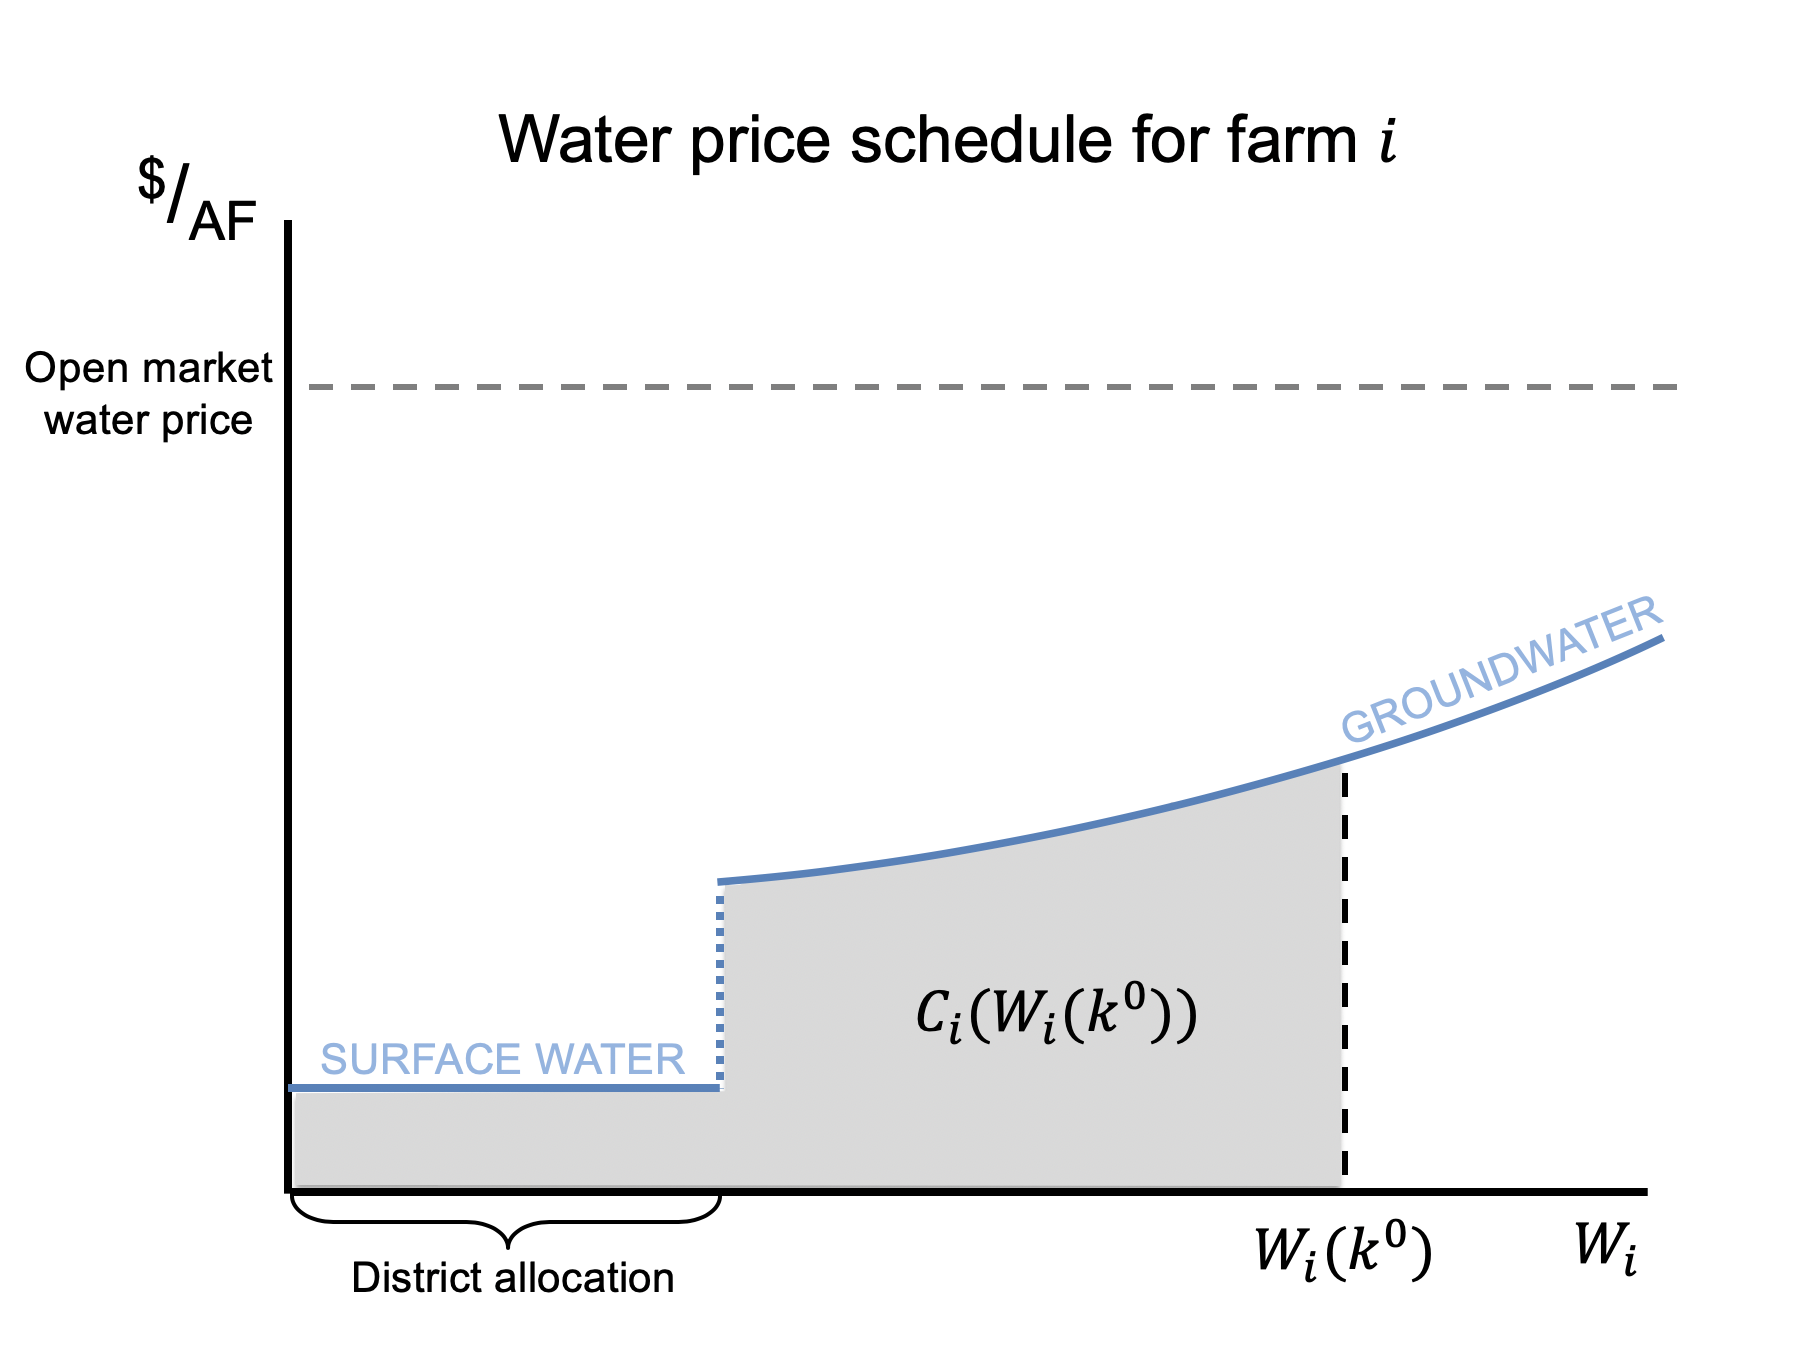
\includegraphics[width=0.495\textwidth, trim={4mm 0 11mm 0mm}, clip]{Figures/water_cost_1.png}
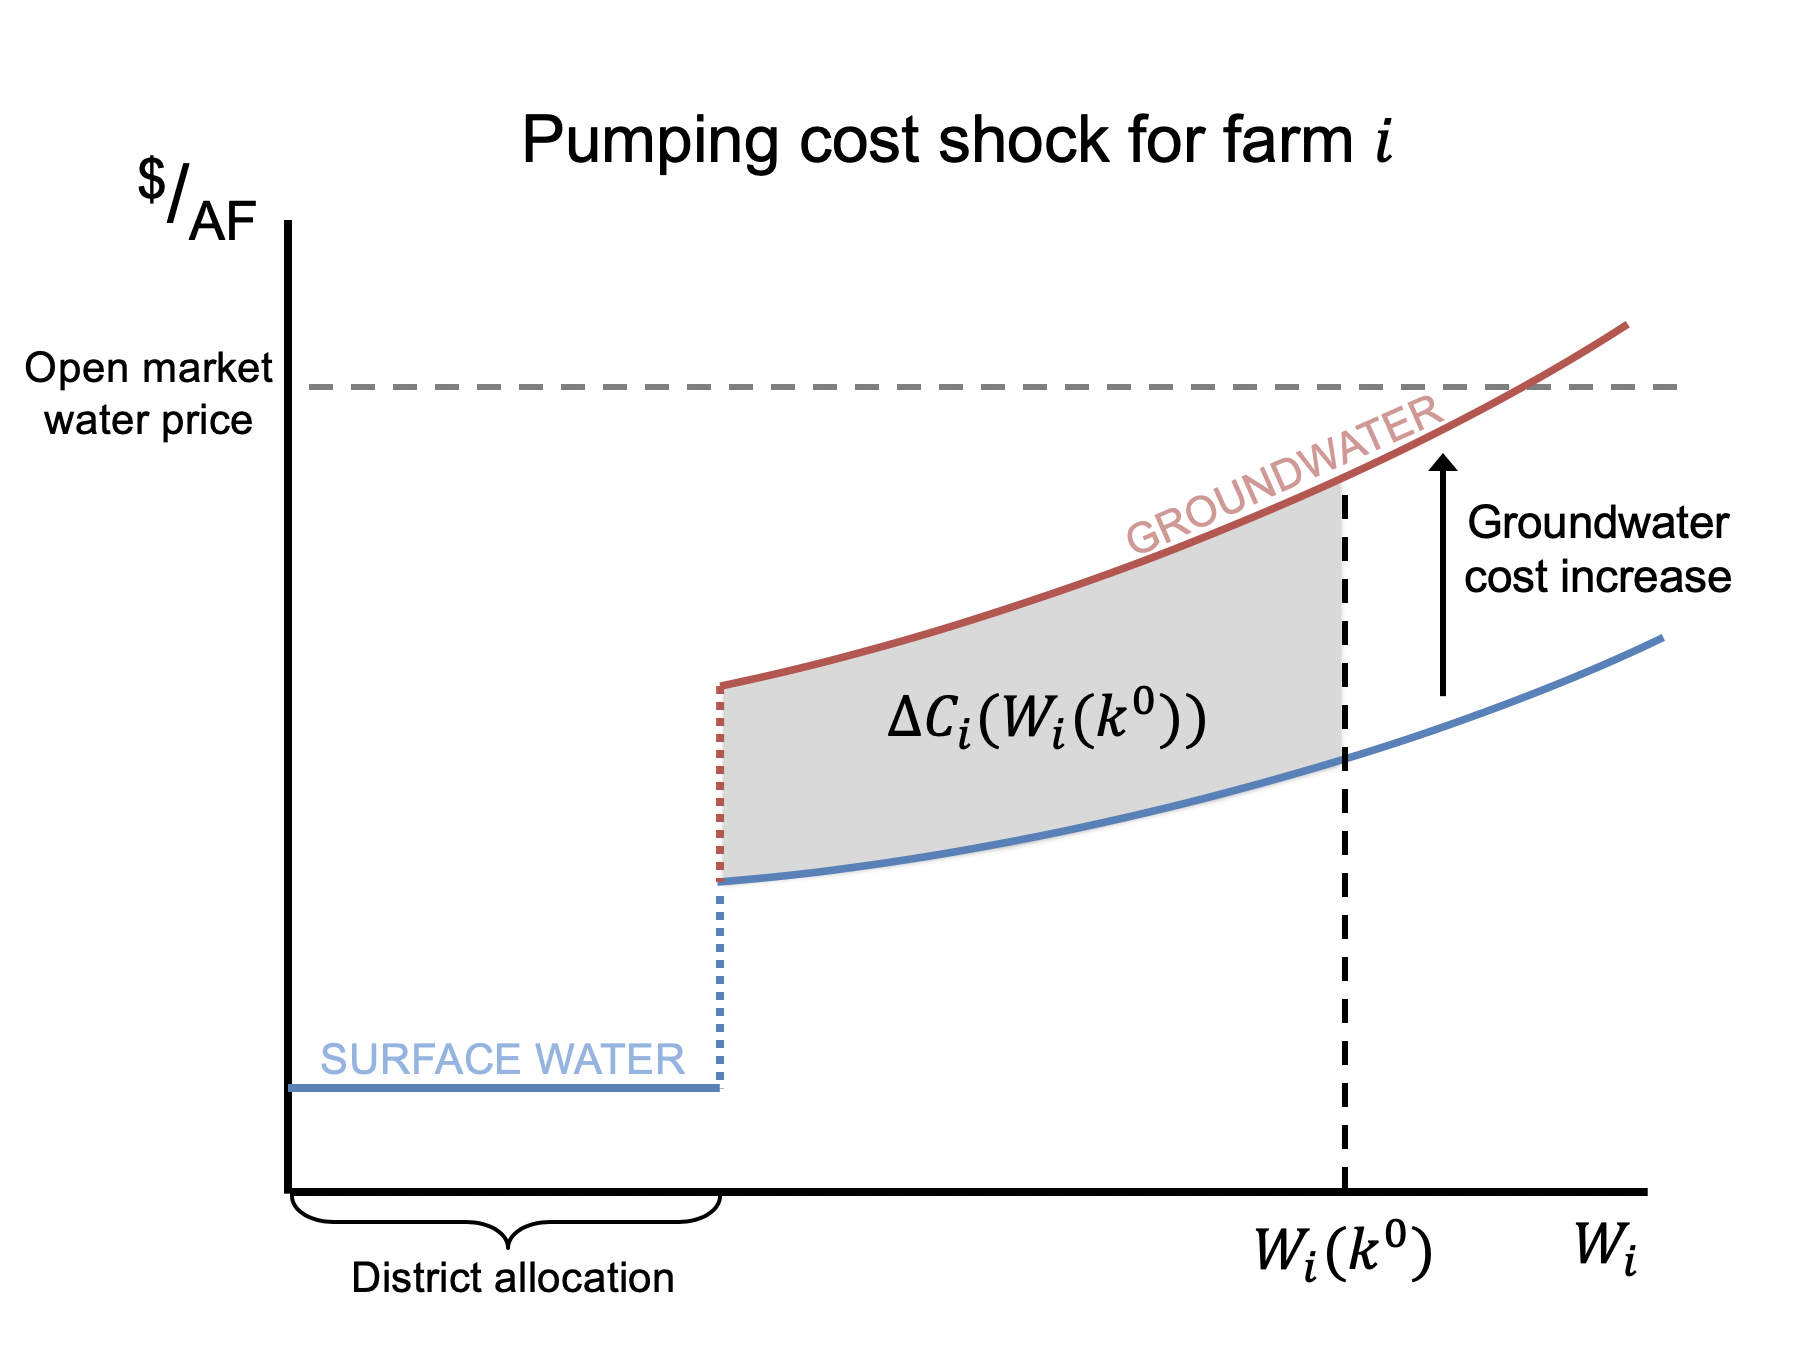
\includegraphics[width=0.495\textwidth, trim={4mm 0 11mm 0mm}, clip]{Figures/water_cost_2.png} \\
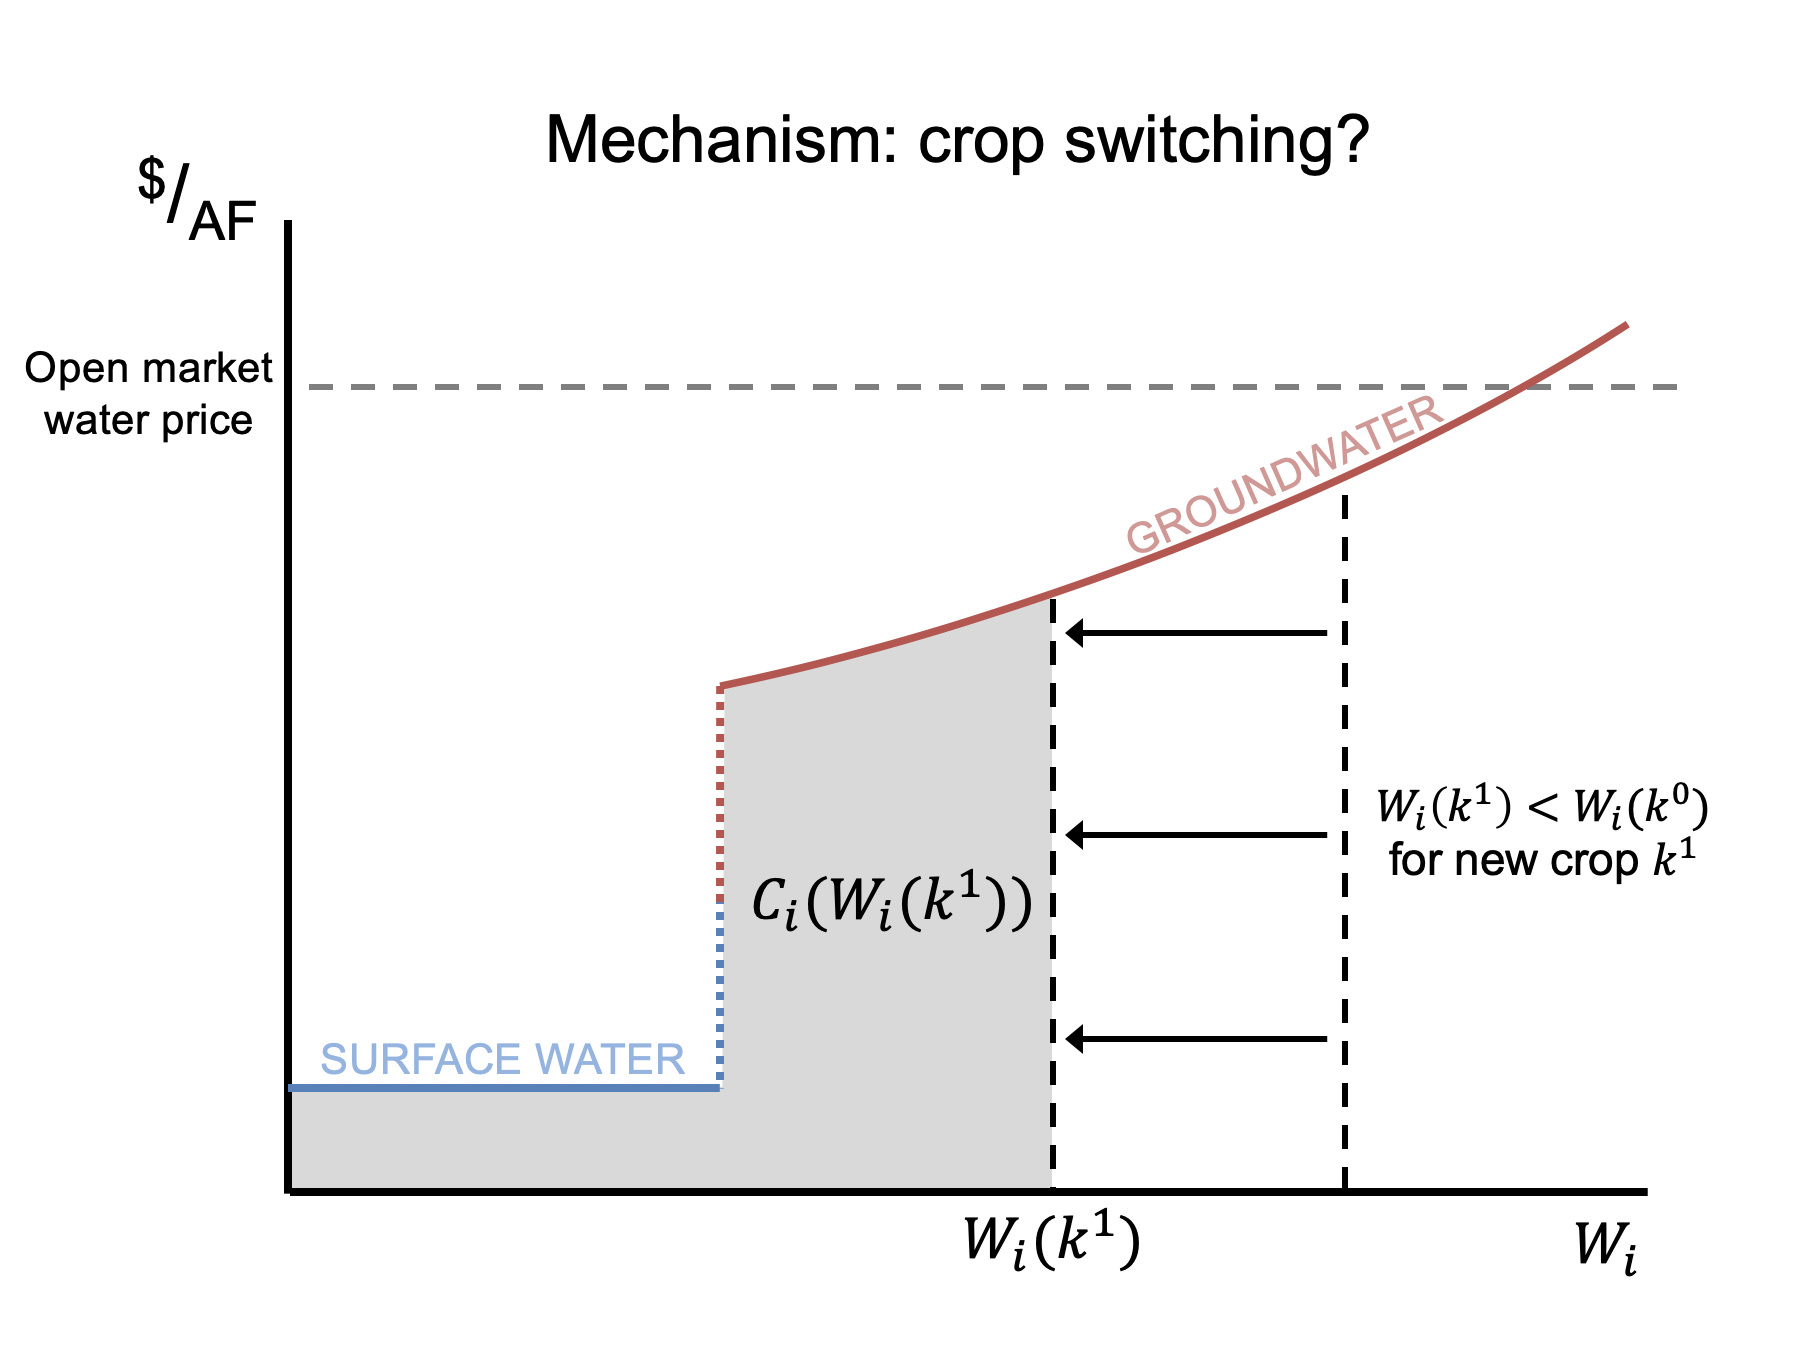
\includegraphics[width=0.495\textwidth, trim={4mm 0 11mm 0mm}, clip]{Figures/water_cost_3.png}
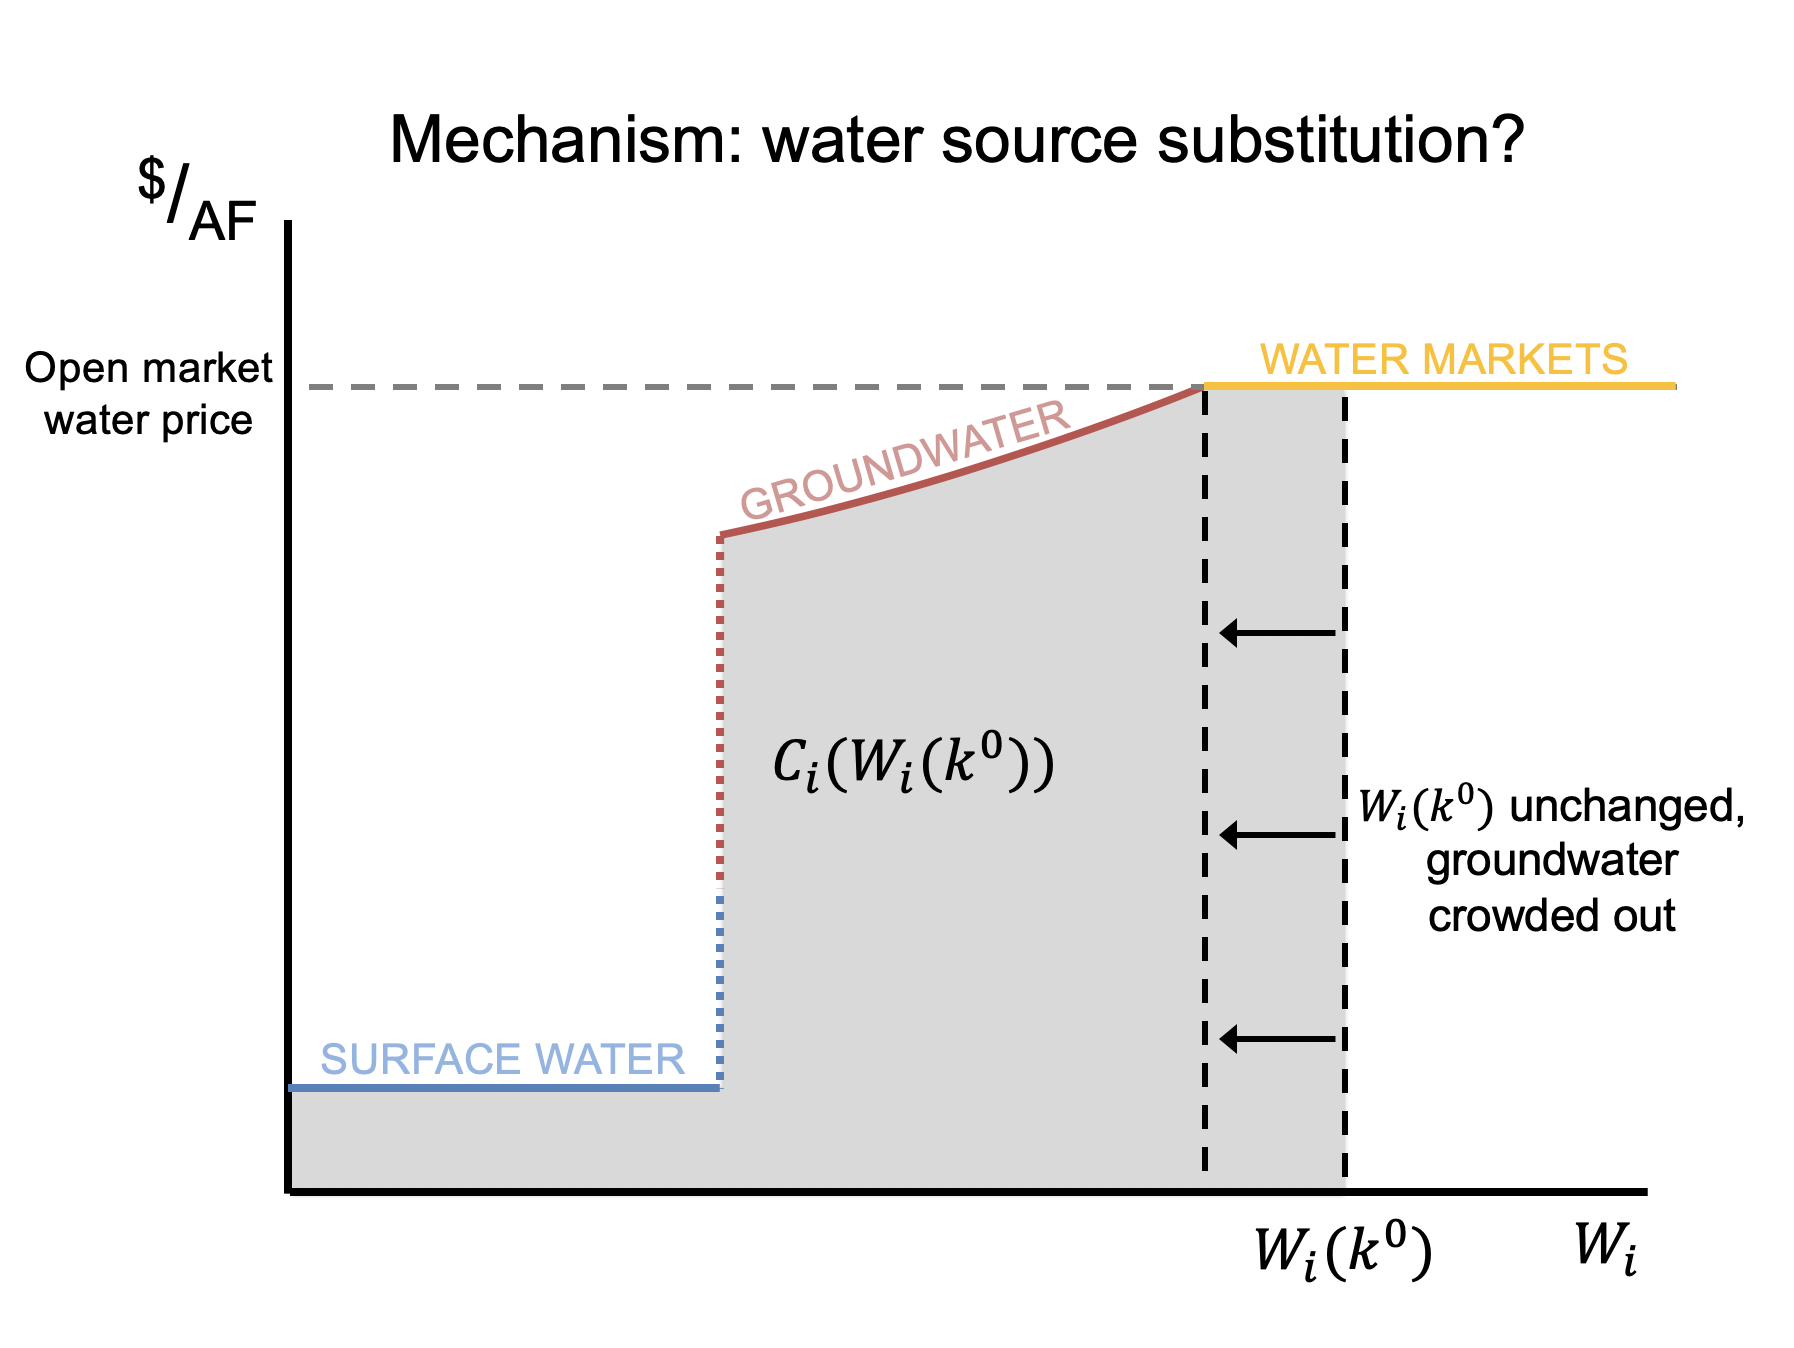
\includegraphics[width=0.495\textwidth, trim={4mm 0 11mm 0mm}, clip]{Figures/water_cost_4.png}
\caption*{\scriptsize \emph{Notes:} This figure presents a stylized water price schedule for a representative farm $i$. The price schedule is nonlinear and comprises water from up to three sources: (i) a low-cost allocation of surface water from farm $i$'s irrigation district; (ii) medium-cost groundwater pumping, with costs that rise gradually in own extraction; and (iii) a high-cost backstop of open market water transactions, for which we assume farm $i$ is a price taker. For crop $k^0$ requiring $W_i(k^0)$ acre/feet of water, farm $i$'s irrigation costs $C_i\big(W_i(k^0)\big)$ are represented by the shaded region in the top-left panel. If farm $i$ experiences a pumping cost shock (due to either an electricity price increase or a groundwater depth increase), its groundwater costs shift up and its total irrigation costs increase by the shaded region $\Delta C_i\big(W_i(k^0)\big)$ in the top-right panel. The bottom panels illustrate two ways that this pumping cost shock increase translate to a reduction in farm $i$'s groundwater consumption. First, the farmer may respond to this pumping cost shock by switching from crop $k^0$ to a less water intensive crop $k^1$, as in the bottom-left panel. Second, for a large enough cost shock, the farmer may continue to grow crop $k^0$, but substitute away from groundwater using open market water purchases.
}
\end{centering}
\end{figure}